%--------------------------------------------------------------------------------------------------
% introduction.tex
%
% This document define the frontespiece of the presentation
%
% author: Andrea Meneghinello
% version: 0.1
%--------------------------------------------------------------------------------------------------
\section{Infrastructure management}
\begin{frame}{Infrastructure management}
	\only<1>
	{
		\begin{columns}
			\begin{column}{0.6\textwidth}
				can be supervised by
				\begin{itemize}
					\item{\footnotesize{business organizations (customers)}}
					\begin{itemize}
						\item{\scriptsize{may not be able to afford qualified personnel}}
						\item{\scriptsize{may not be able to afford dedicated hardware}}
						\item{\scriptsize{higher cost}}
					\end{itemize}
				\end{itemize}
			\end{column}
			\begin{column}{0.4\textwidth}
				\begin{figure}
					\centering{}
					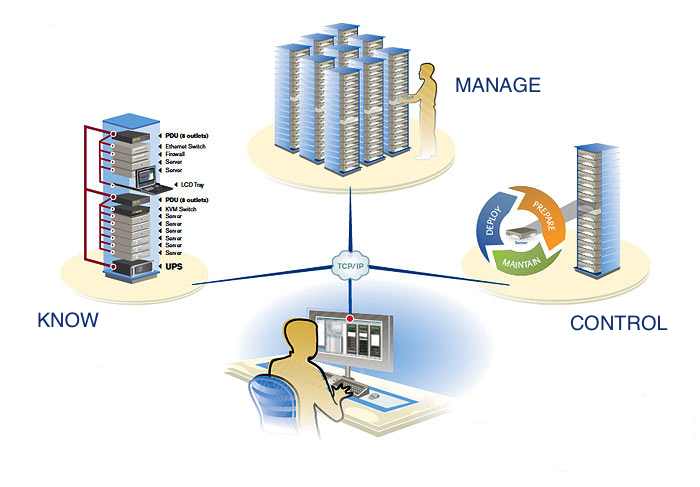
\includegraphics[scale=0.2]{images/scenarios.png}
				\end{figure}
				\begin{flushright}
					\tiny{source: \url{http://goo.gl/IiVnC6}}
				\end{flushright}
			\end{column}
		\end{columns}
	}
	\only<2>
	{
		\begin{columns}
			\begin{column}{0.6\textwidth}
				can be supervised by
				\begin{itemize}
					\item{\footnotesize{providers (suppliers)}}
					\begin{itemize}
						\item{\scriptsize{manage \textit{n} different infrastructures}}
						\begin{itemize}
							\item{\tiny{integrate - adapt - maintain}}
						\end{itemize}
						\item{\scriptsize{higher cost of dedicated personnel}}
						\item{\scriptsize{have to deliver more quantity and value for less time and cost}}
						\item{\scriptsize{have to respect agreed Service Level Agreement (SLA) with customers}}
					\end{itemize}
				\end{itemize}
			\end{column}
			\begin{column}{0.4\textwidth}
				\begin{figure}
					\centering{}
					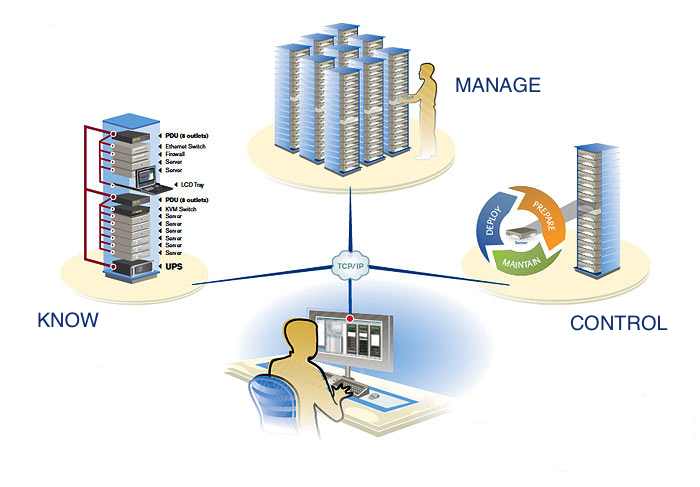
\includegraphics[scale=0.2]{images/scenarios.png}
				\end{figure}
				\begin{flushright}
					\tiny{source: \url{http://goo.gl/IiVnC6}}
				\end{flushright}
			\end{column}
		\end{columns}
	}
\end{frame}

\subsection{Cloud characteristics}
\begin{frame}{Cloud characteristics}
	\begin{columns}
		\begin{column}{0.5\textwidth}
			customers look for
			\begin{itemize}
				\item{\footnotesize{on-demand self-service}}
				\item{\footnotesize{web-based access}}
				\item{\footnotesize{rapid \textbf{elasticity}}}
				\item{\footnotesize{pay-as-you-go model}}
			\end{itemize}
			providers look for
			\begin{itemize}
				\item{\footnotesize{resource pooling}}
				\item{\footnotesize{rapid \textbf{elasticity}}}
			\end{itemize}
		\end{column}
		\begin{column}{0.5\textwidth}
			\begin{figure}
				\centering{}
				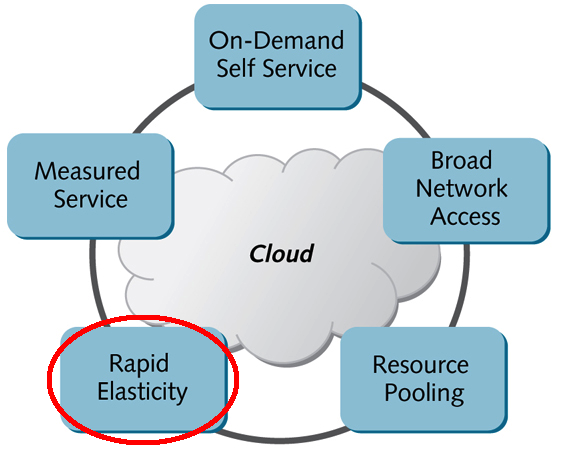
\includegraphics[scale=0.25]{images/cloud-characteristics-selected.png}
			\end{figure}
			\begin{flushright}
				\tiny{source: \url{http://goo.gl/pF2xPw}}
			\end{flushright}
		\end{column}
	\end{columns}
\end{frame}

\subsection{SPI stack}
\begin{frame}{SPI stack}
	\begin{columns}
		\begin{column}{0.6\textwidth}
			current focus on elasticity management on
			\begin{itemize}
				\item{\footnotesize{Infrastructure as a Service (IaaS)}}
				\item{\footnotesize{Software as a Service (SaaS)}}
			\end{itemize}
			in clear conflict of interest
			\begin{center}
				$\downarrow{}$\\a mediator is needed $\rightarrow{}$ PaaS
			\end{center}
		\end{column}
		\begin{column}{0.3\textwidth}
			\begin{figure}
				\centering{}
				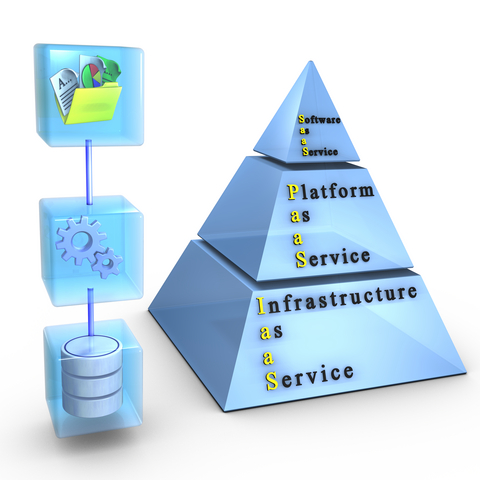
\includegraphics[scale=0.2]{images/spi.png}
			\end{figure}
			\begin{flushright}
				\tiny{source \url{http://goo.gl/QKHPsV}}
			\end{flushright}
		\end{column}
	\end{columns}
\end{frame}

\subsection{Platform as a Service (PaaS)}
\begin{frame}{Platform as a Service (PaaS)}
	\only<1>
	{
		\begin{columns}
			\begin{column}{0.55\textwidth}
				PaaS is
				\begin{itemize}
					\item{\footnotesize{like a middleware}}
					\begin{itemize}
						\item{\scriptsize{transactions - security - clustering}}
						\item{\scriptsize{features provided \textbf{automatically}}}
					\end{itemize}
					\item{\footnotesize{not like a middleware}}
					\begin{itemize}
						\item{\scriptsize{no static SW $\rightarrow{}$ no manual configuration}}
					\end{itemize}
					\item{\footnotesize{manage Units of Deployments (UoD)}}
				\end{itemize}
			\end{column}
			\begin{column}{0.45\textwidth}
				\begin{figure}
					\centering{}
					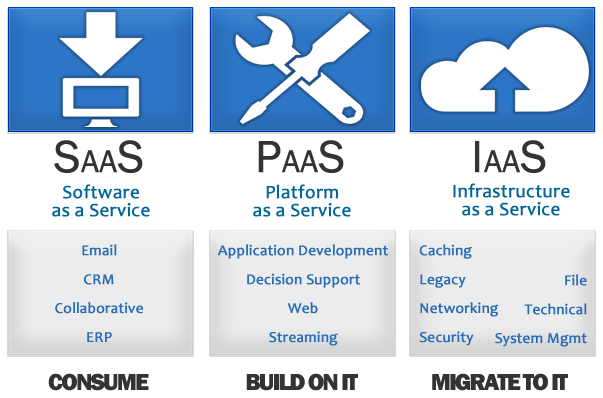
\includegraphics[scale=0.22]{images/paas.png}
				\end{figure}
				\begin{flushright}
					\tiny{source: \url{http://goo.gl/iHwYsH}}
				\end{flushright}
			\end{column}
		\end{columns}
	}
	\only<2>
	{
		\begin{figure}
			\centering{}
			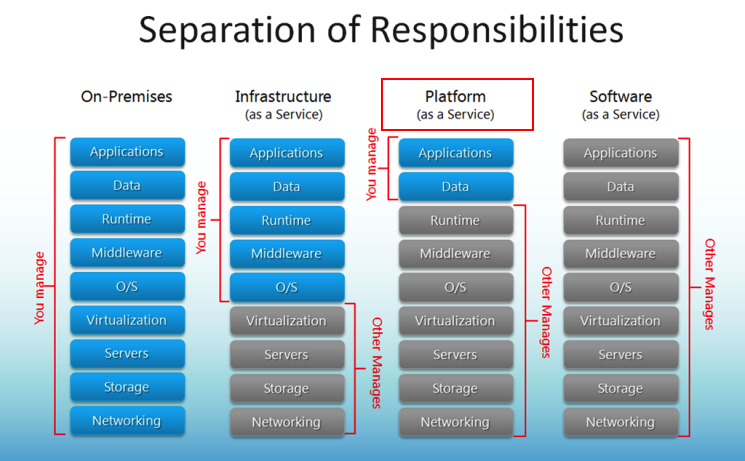
\includegraphics[scale=0.33]{images/separation-responsabilities.png}
		\end{figure}
		\begin{flushright}
			\tiny{source: \url{http://goo.gl/YUw1jW}}
		\end{flushright}
	}
\end{frame}

\subsection{Units of Deployments}
\begin{frame}{Units of Deployments (UoD)}
	\only<1>
	{
		\begin{columns}
			\begin{column}{0.7\textwidth}
				available
				\begin{itemize}
					\item{\footnotesize{Virtual Machines (VMs)}}
					\item{\footnotesize{Containers}}
				\end{itemize}
				virtualization interfaces
				\begin{itemize}
				\item{\footnotesize{VMs $\rightarrow{}$ Instruction Set Architecture (ISA)}}
				\item{\footnotesize{Containers $\rightarrow{}$ Application Binary Interface (ABI)}}
				\end{itemize}
				\begin{center}
					both need a \textbf{hypervisor} to execute
				\end{center}
			\end{column}
			\begin{column}{0.3\textwidth}
				\begin{figure}
					\centering{}
					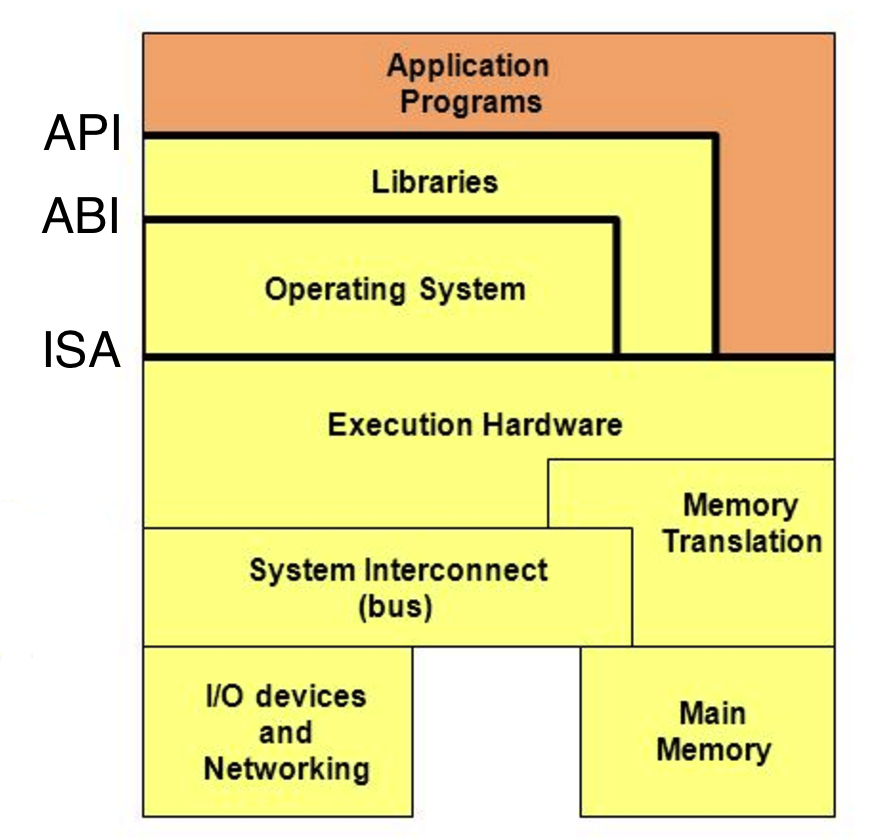
\includegraphics[scale=0.11]{images/virtualization-level.png}
				\end{figure}
				\begin{flushright}
					\tiny{source: \url{http://goo.gl/mya7fi}}
				\end{flushright}
			\end{column}
		\end{columns}
	}
	\only<2>
	{
		\begin{columns}
			\begin{column}{0.7\textwidth}
				\begin{figure}
					\centering{}
					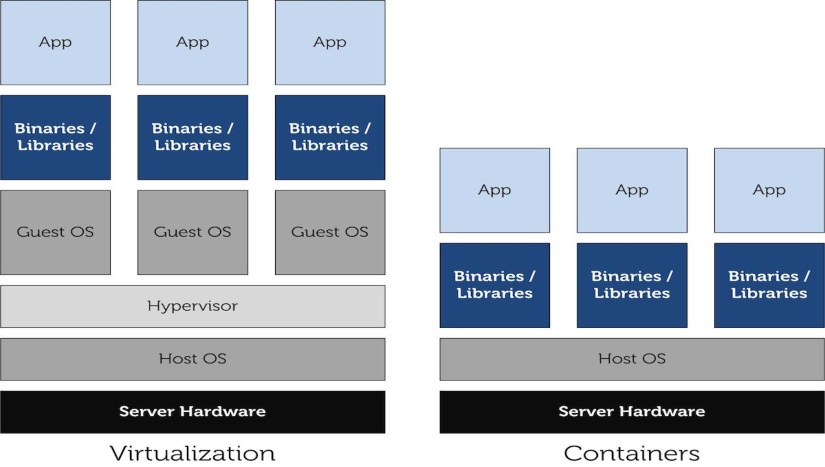
\includegraphics[scale=0.7]{images/containerization.png}
				\end{figure}
				\begin{center}
					\tiny{source: \url{http://goo.gl/CSutcf}}
				\end{center}
			\end{column}
			\begin{column}{0.3\textwidth}
				\begin{figure}
					\centering{}
					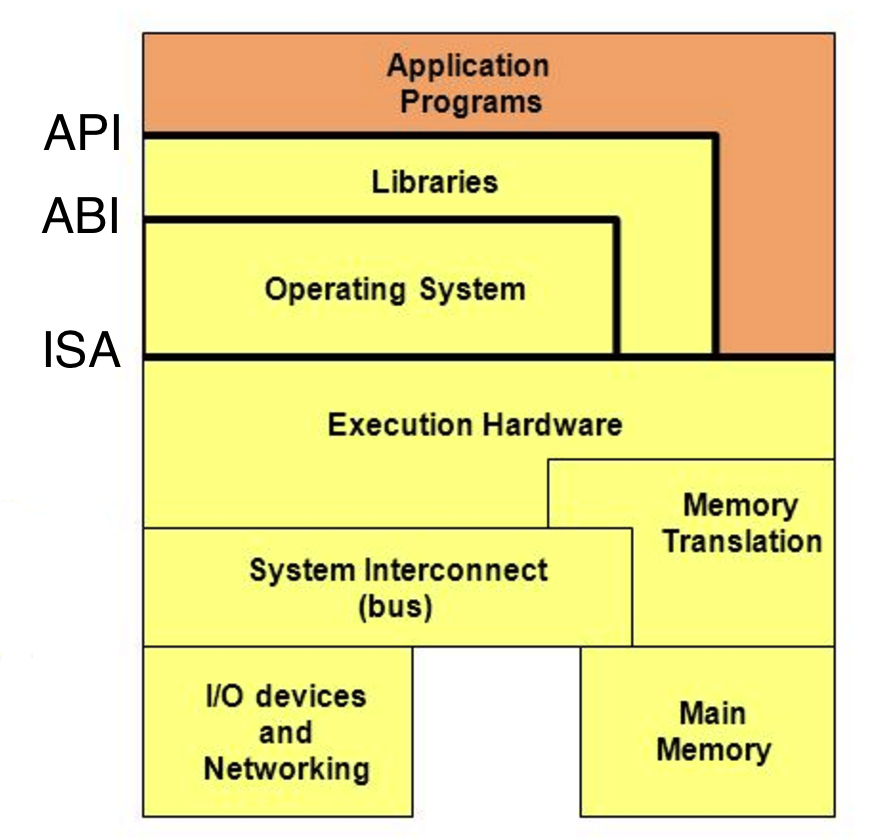
\includegraphics[scale=0.1]{images/virtualization-level.png}
				\end{figure}
				\begin{flushright}
					\tiny{source: \url{http://goo.gl/mya7fi}}
				\end{flushright}
			\end{column}
		\end{columns}
	}
\end{frame}

\subsection{Docker containers}
\begin{frame}{Docker containers}
	\only<1>
	{
		\begin{columns}
			\begin{column}{0.5\textwidth}
				characteristics
				\begin{itemize}
					\item{\footnotesize{born off LinuX Containers (LXC)}}
					\item{\footnotesize{client-server architecture}}
					\item{\footnotesize{data management}}
					\begin{itemize}
						\item{\scriptsize{Union File System (UFS)}}
						\item{\scriptsize{data volumes}}
						\item{\scriptsize{data volume containers}}
					\end{itemize}
					\item{\footnotesize{manage ``dependency-hell'' problem}}
				\end{itemize}
			\end{column}
			\begin{column}{0.5\textwidth}
				\begin{figure}
					\centering{}
					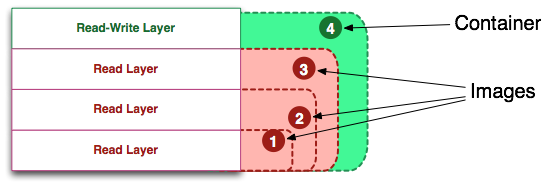
\includegraphics[scale=0.3]{images/union-fs.png}
				\end{figure}
				\begin{flushright}
					\tiny{source: \url{http://goo.gl/8nEkSc}}
				\end{flushright}
			\end{column}
		\end{columns}
	}
	\only<2>
	{
		\begin{figure}
			\centering{}
			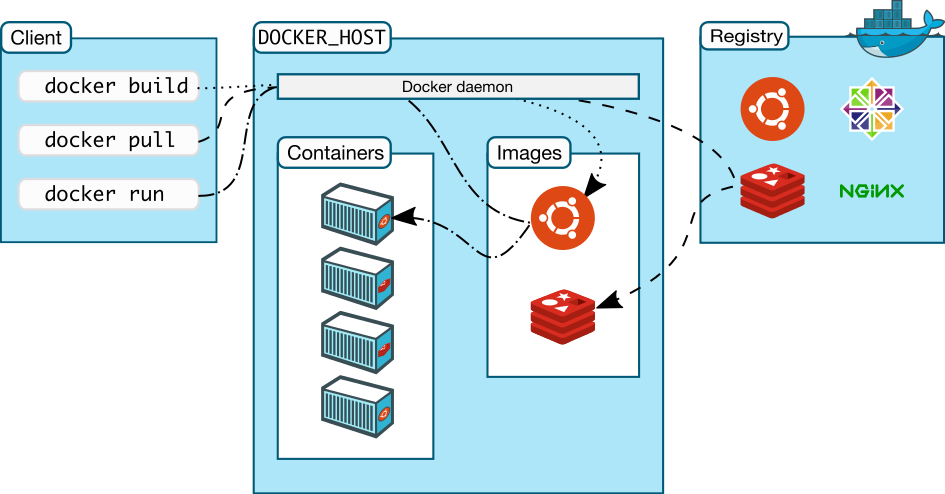
\includegraphics[scale=0.35]{images/docker-architecture.png}
		\end{figure}
		\begin{flushright}
			\tiny{source: \url{https://goo.gl/7UXgAa}}
		\end{flushright}
	}
\end{frame}